\documentclass[a4paper,12pt]{article}
\usepackage{amssymb,amsmath,amsfonts,amsbsy}
\usepackage{graphicx}
\usepackage{numprint}
\usepackage{tabularx}
\usepackage{setspace}
\usepackage{authblk}
\usepackage{longtable}
\usepackage{setspace}
\usepackage{rotating}
\usepackage{float}
\usepackage{censor,caption}
\usepackage{enumitem}
\usepackage{tikz} % package p r i n c i p a l TikZ
\usetikzlibrary{shapes.geometric}
\usetikzlibrary{shapes}
\usepackage{color}
\usepackage{soul}
\usepackage[left=3cm,right=3cm,top=3cm,bottom=3cm]{geometry}
\usepackage{listings}
%\usepackage[style=authoryear-icomp,sortcites=true,sorting=nyt,backend=bibtex]{biblatex}
%\addbibresource{bibliography.bib}

\title{Supplementary materials: Are Bayesian Regularization Methods a Must for Multilevel Dynamic Latent Variables Models?}
\author{}
\date{}

\begin{document}
\maketitle

We provide here supplementary materials containing results that are not shown in the manuscript for simulation study 1 and simulation study 2. We present here several graphics showing the small sample properties of the estimates. In particular, we illustrated the convergence rates and the sampling precision rates across data conditions. We also computed the absolute bias, the relative bias as well as the root mean squared error (RMSE). Their behavior across the data conditions are shown here. Furthermore, in the manuscript we only presented the type-I-error rates and the NDR when 50\% of the components of the vector of slopes $\pmb{\beta}$ are zeros. In this document, we presented these metrics when 75\% of $\pmb{\beta}$'s components are zeros.

\section{Simulation study 1}

\subsection*{Convergence rates and sampling precision rates}
\paragraph{Convergence}
Here, we describes the convergence rates across replications and the data conditions. We say that a model converge if we have $\text{R-hat}>1.1$ for each parameter of the model. \\
 
\begin{figure}[h]
\centering 
\label{fig:CVr_nz25}
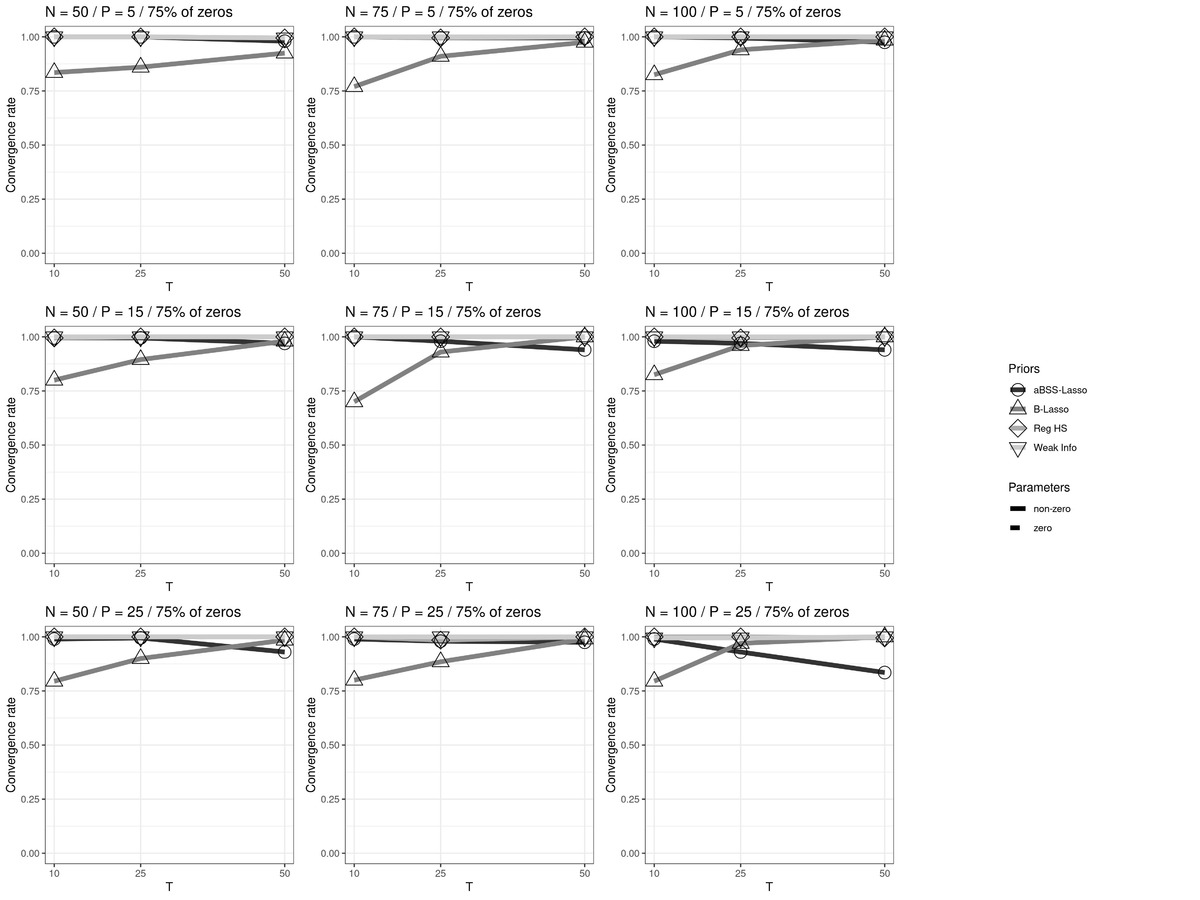
\includegraphics[width=18cm]{CVr_nz25_beta.jpg}
\caption{Convergence rates (based on $\text{R-hat}>1.1$) across $N, T$ and $P$ when 75\% of $\beta$ components are zeros}
\end{figure}

\begin{figure}[]
\centering 
\label{fig:CVr_nz50}
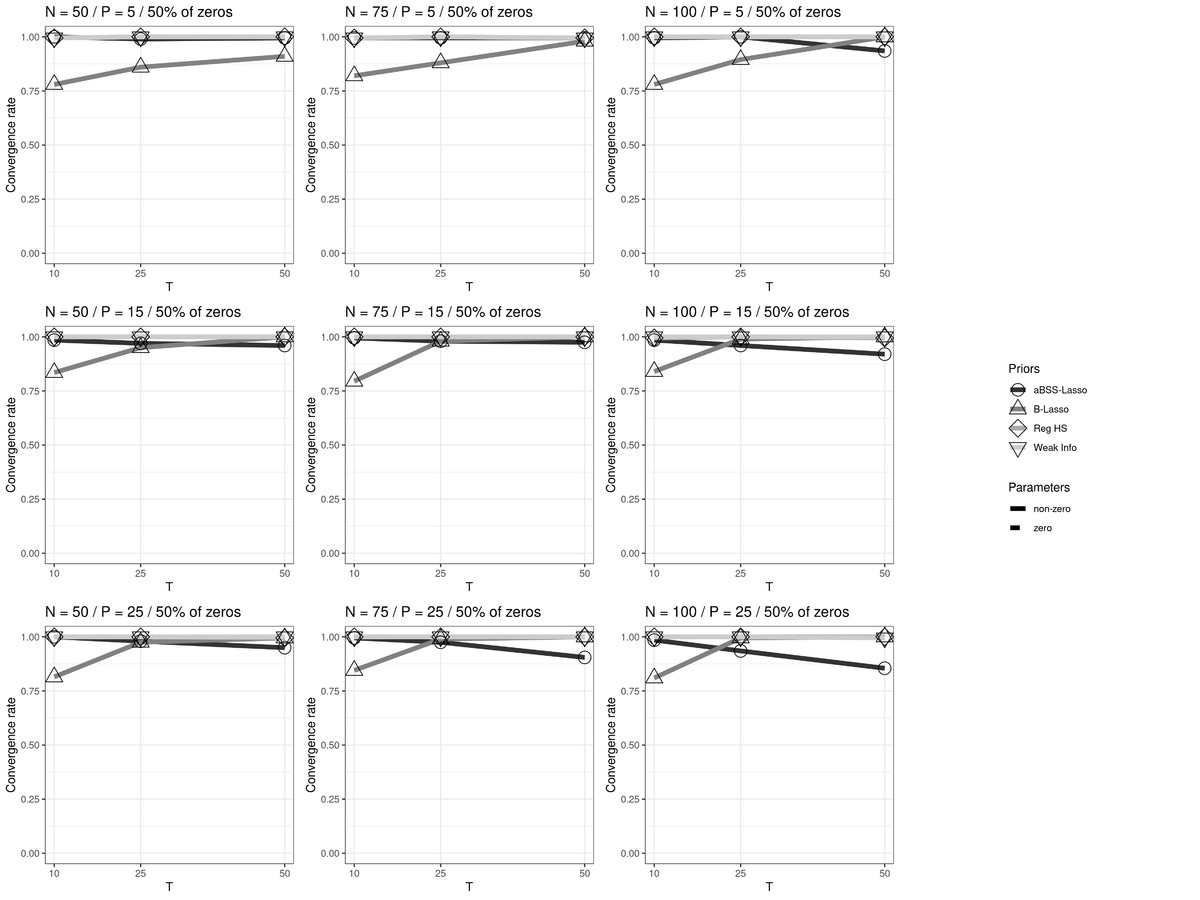
\includegraphics[width=18cm]{CVr_nz50_beta.jpg}
\caption{Convergence rates (based on $\text{R-hat}>1.1$) across $N, T$ and $P$ when 50\% of $\beta$ components are zeros}
\end{figure}

\clearpage
\paragraph{Sampling Precision}
We also calculated the sampling precision based on the threshold over the effective sample size (ESS). These thresholds are $x = 100, 400, 1000$. The precision rates are calculated across replications, so that for a given replication, if all parameters had $ESS > x$, then we say that the HMC sampling applied to that replication provided the expected sampling precision.

First, Figures \ref{fig:Prec100_nz25} and \ref{fig:Prec100_nz50} show the precision rates when model parameters have $ESS > 100$. The weakly informative prior provided a precision rate above 99\%, with an average precision rate of 99.8\% across all data conditions. For the Reg HS, the lowest precision rate was 97.5\% and the average precision rate across data conditions was 99.6\%. For the aBSS-lasso prior, the lowest precision rate was 76\% with an average rate of 94.7\% across data conditions. For the B-Lasso prior, the lowest precision rate was 51.5\% and the average rate across data conditions was 82.7\%. Note that for the B-Lasso prior, precision rates were particularly low when the length of time points $T$ was small. As shown in the figures, larger $T$ were needed to increase these precision rates. Second, Figures \ref{fig:Prec400_nz25} and \ref{fig:Prec400_nz50} show the precision rates when model parameters have $ESS > 400$. The weakly informative priors (with an average precision rate of 98.5\% and a minimum precision rate of 92\%) and the Reg HS (with an average precision rate of 98.1\% and a minimum precision rate of 95\%) had the best precision rate. The aBSS-Lasso prior provided lower precision with respect to $x = 400$ (with an average rate of 86.4\% and a minimum rate of 86.4\%) The B-Lasso prior performed the worst at this threshold. As shown in figures, larger $N$ and $T$ were required to cope with the increase in $P$. Third, in Figures \ref{fig:Prec1000_nz25} and \ref{fig:Prec1000_nz50}, we also provided the precision rates when all model parameters have $ESS > 1000$. Despite the low precision rates for the B-Lasso priors shown earlier, we observed that the precision rates are very high with $x = 100$, which can reach 100\% when N can reach 100\% when $N = 100$. \\

\begin{figure}[h]
\centering 
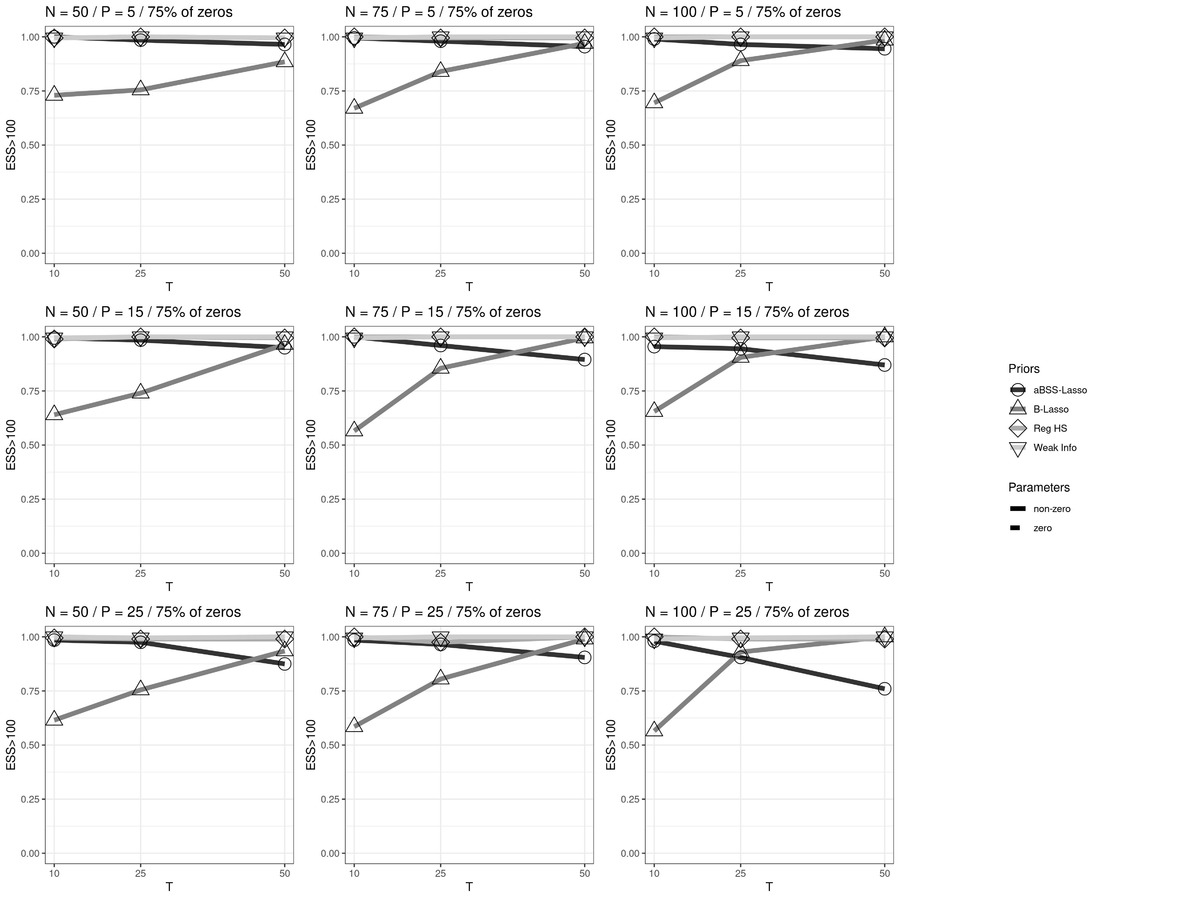
\includegraphics[width=18cm]{Prec100_nz25_beta.jpg}
\caption{Sampling precision rates (based on $ESS>100$) across $N, T$ and $P$ when 75\% of $\beta$ components are zeros}
\label{fig:Prec100_nz25}
\end{figure}

\begin{figure}[]
\centering 
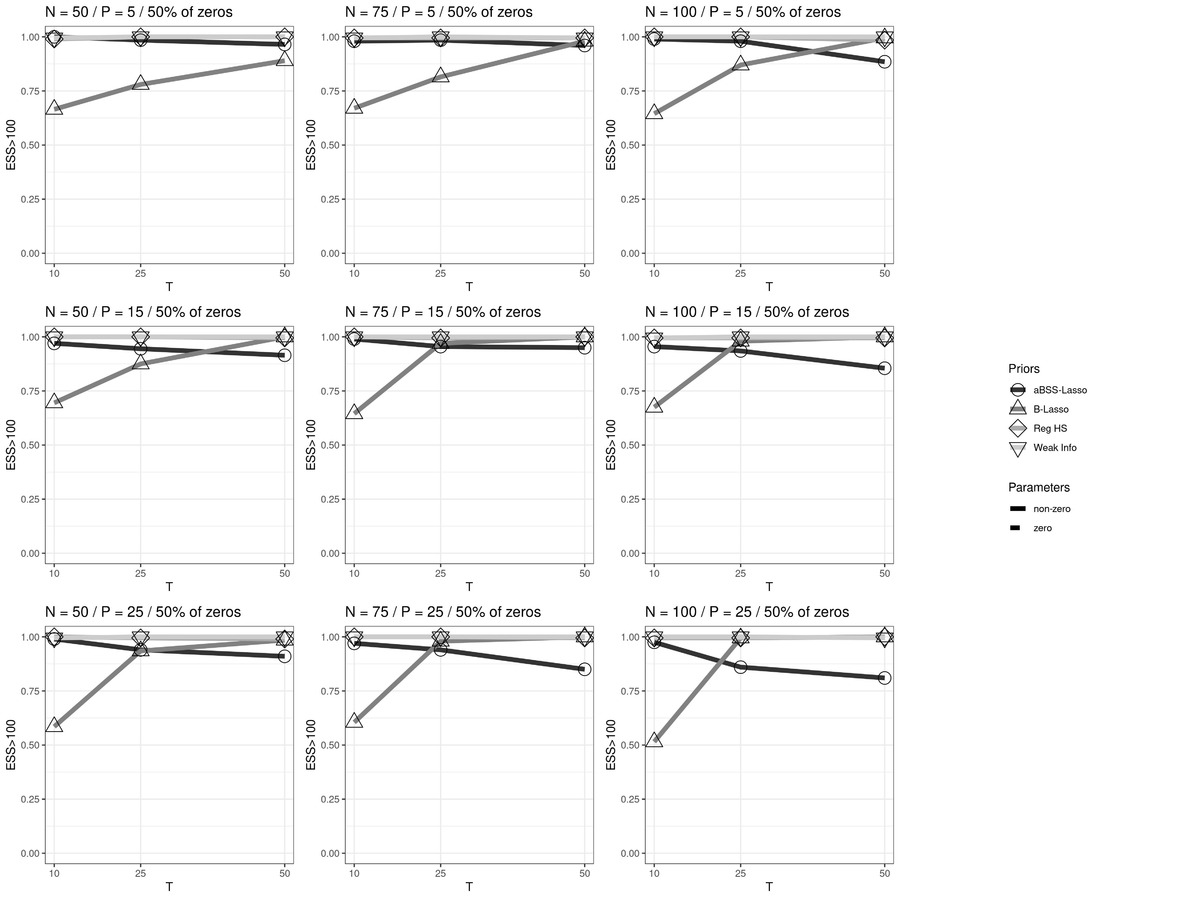
\includegraphics[width=18cm]{Prec100_nz50_beta.jpg}
\caption{Sampling precision rates (based on $ESS>100$) across $N, T$ and $P$ when 50\% of $\beta$ components are zeros}
\label{fig:Prec100_nz50}
\end{figure}

\clearpage
\begin{figure}[]
\centering 
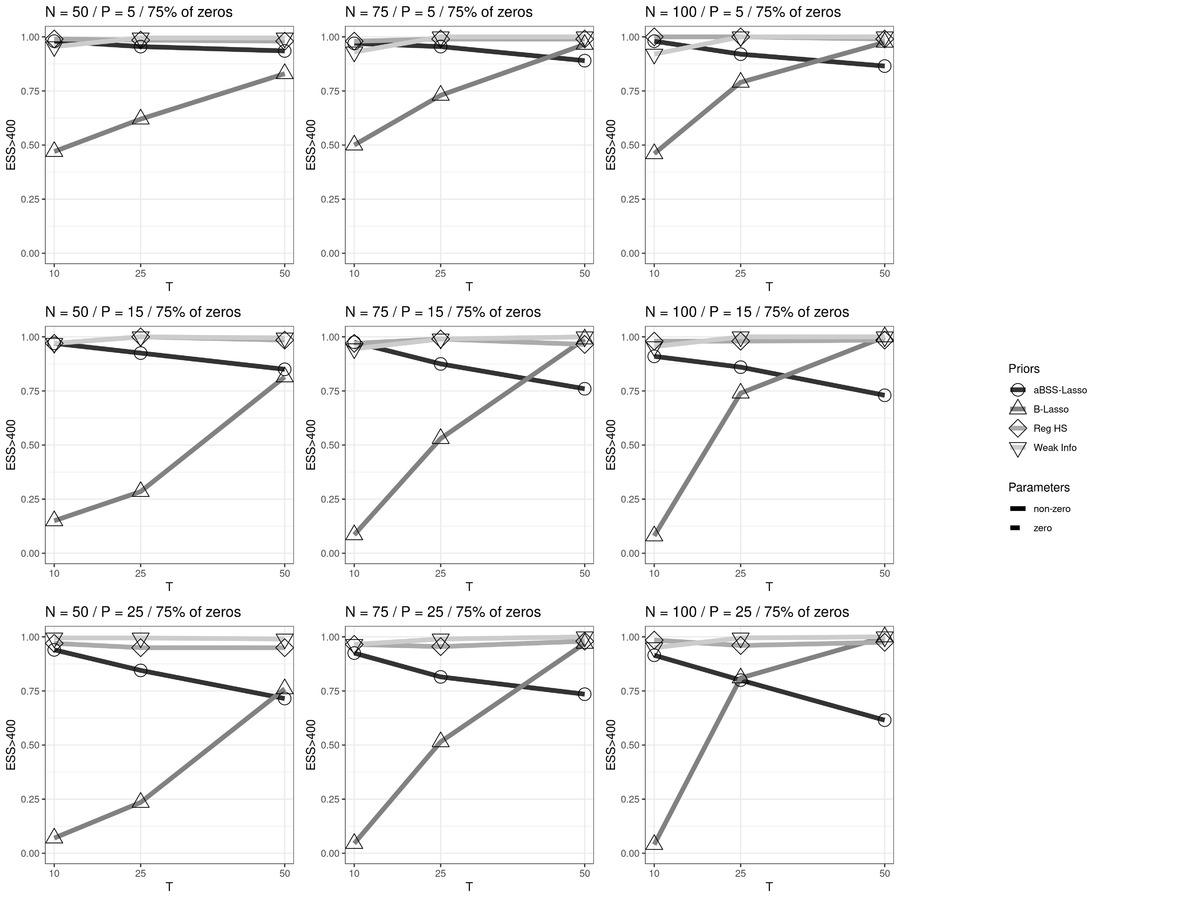
\includegraphics[width=18cm]{Prec400_nz25_beta.jpg}
\caption{Sampling precision rates (based on $ESS>400$) across $N, T$ and $P$ when 75\% of $\beta$ components are zeros}
\label{fig:Prec400_nz25}
\end{figure}

\begin{figure}[]
\centering 
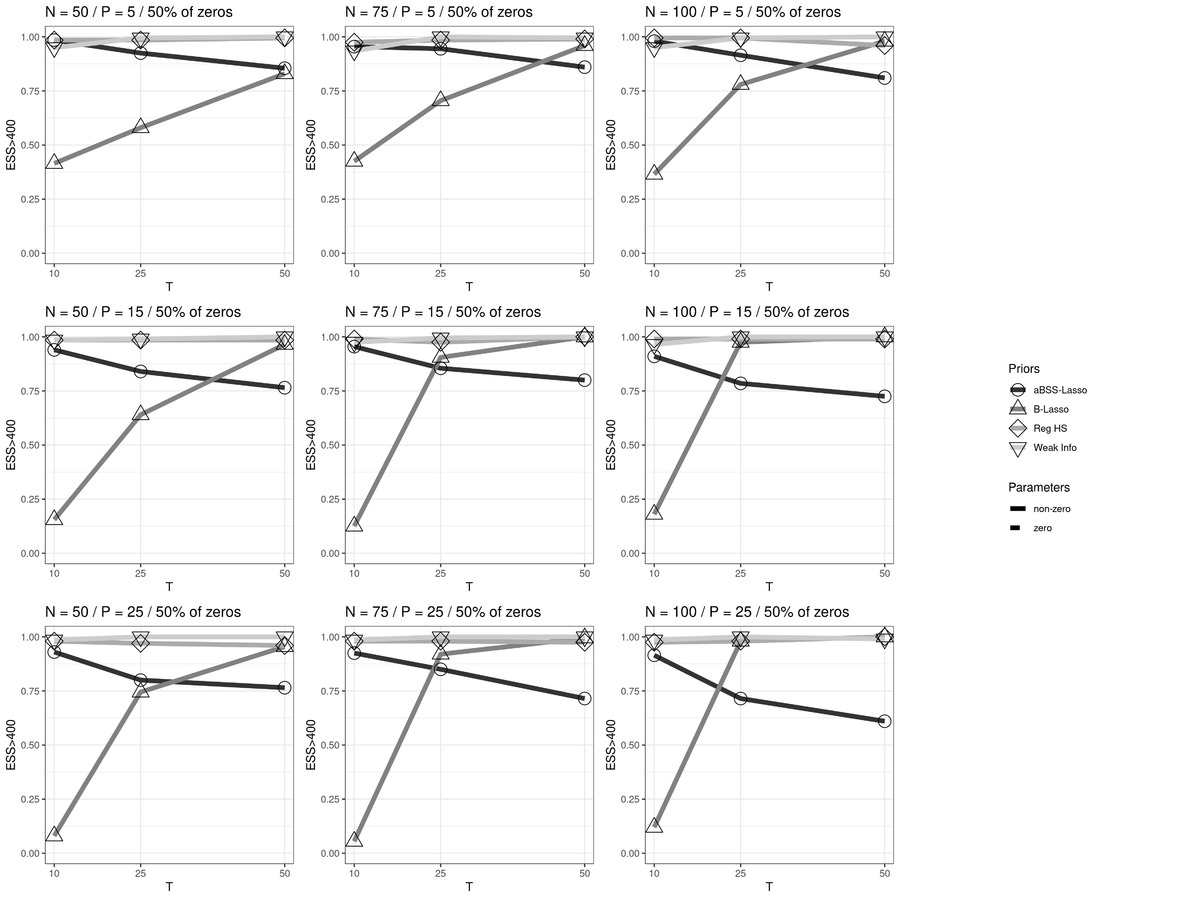
\includegraphics[width=18cm]{Prec400_nz50_beta.jpg}
\caption{Sampling precision rates (based on $ESS>400$) across $N, T$ and $P$ when 50\% of $\beta$ components are zeros}
\label{fig:Prec400_nz50}
\end{figure}

\clearpage
\begin{figure}[]
\centering 
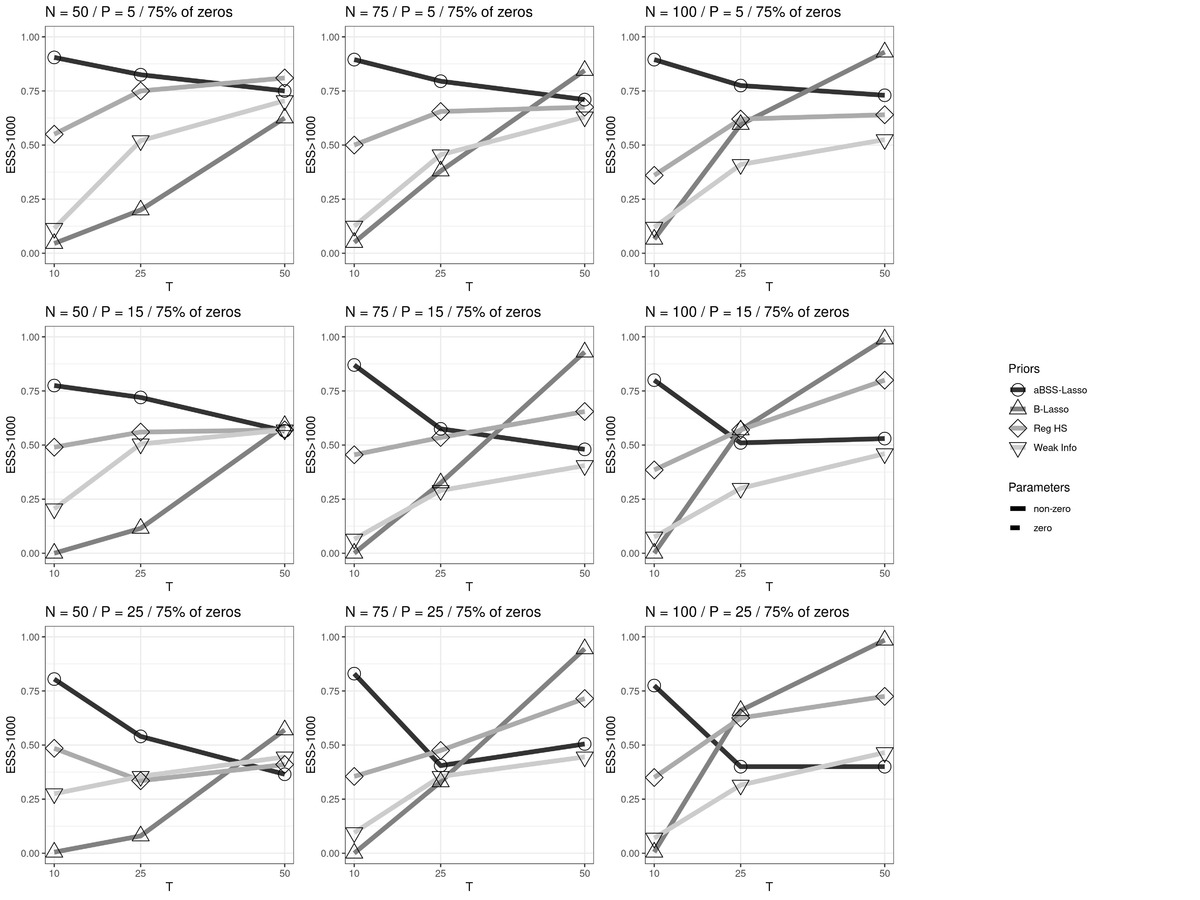
\includegraphics[width=18cm]{Prec1000_nz25_beta.jpg}
\caption{Sampling precision rates (based on $ESS>1000$) across $N, T$ and $P$ when 75\% of $\beta$ components are zeros}
\label{fig:Prec1000_nz25}
\end{figure}

\begin{figure}[]
\centering 
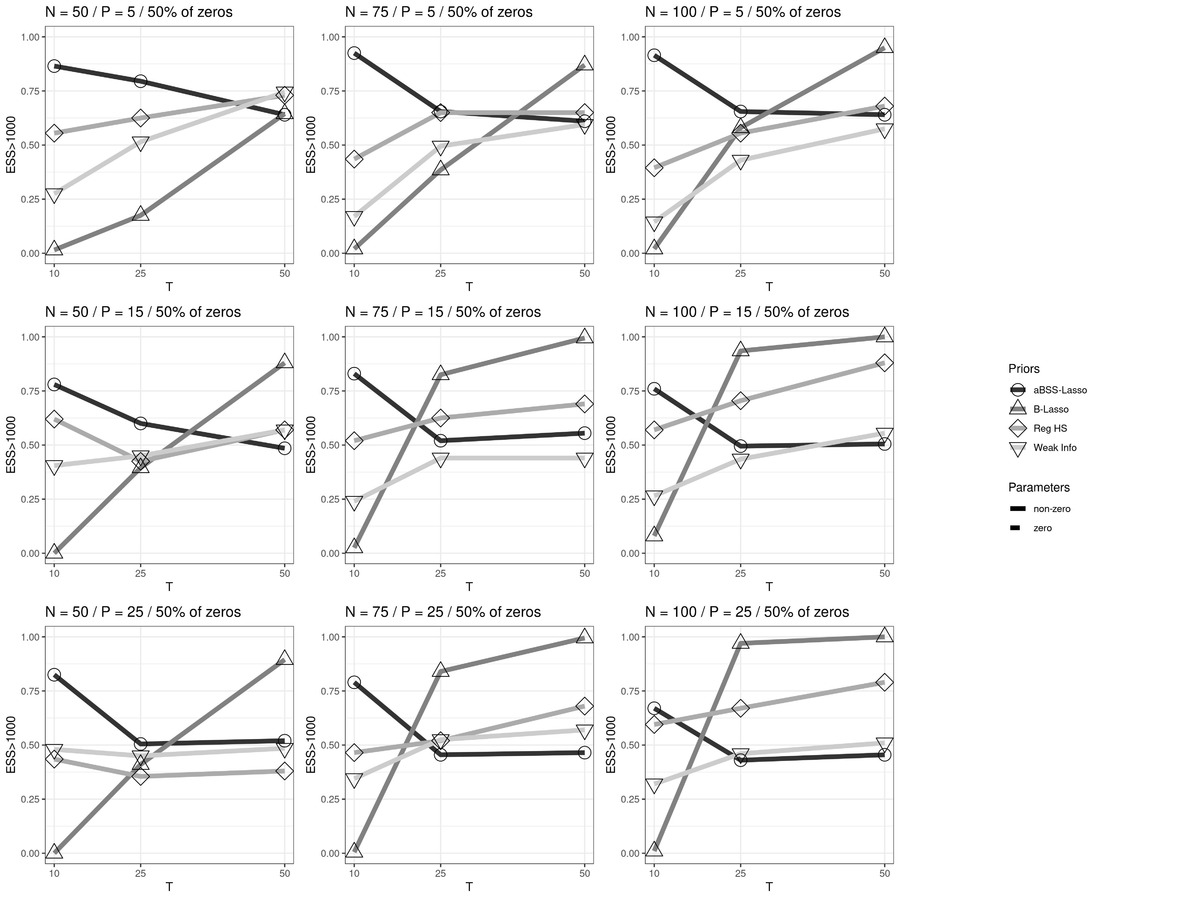
\includegraphics[width=18cm]{Prec1000_nz50_beta.jpg}
\caption{Sampling precision rates (based on $ESS>1000$) across $N, T$ and $P$ when 50\% of $\beta$ components are zeros}
\label{fig:Prec1000_nz50}
\end{figure}

\clearpage
\subsection*{Finite sample properties}
\paragraph*{Absolute Bias}
The absolute bias of an estimator $\hat{\theta}_m$ of a parameter $\theta$ is computed by the following  quantity:
\[  AB = \frac{1}{M} \sum_{m=1}^{M}|\theta-\hat{\theta}_m| \]

\begin{figure}[h]\label{fig:ABias_nz25}
\centering 
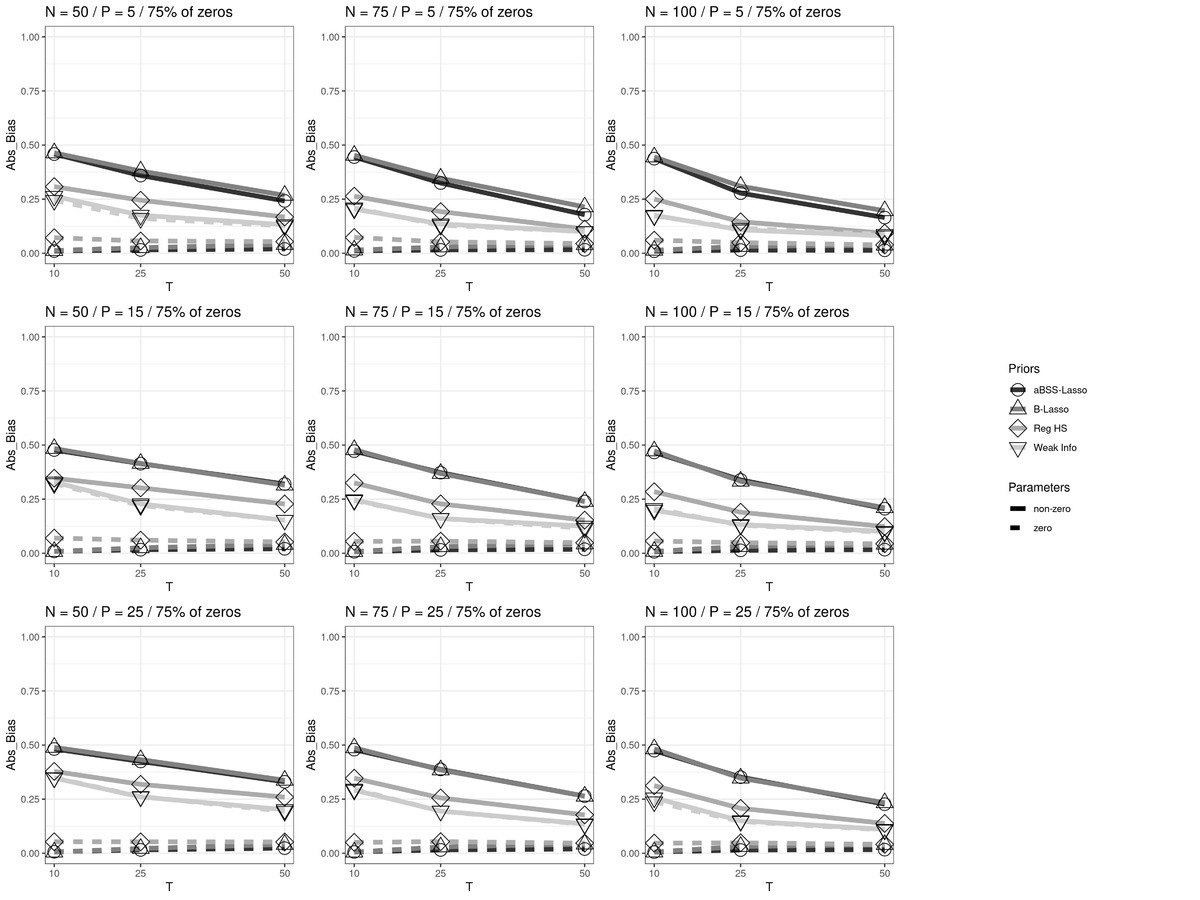
\includegraphics[width=18cm]{Abs_Bias_nz25_beta.jpg}
\caption{Absolute Bias across $N, T$ and $P$ slope when 75\% of $\beta$ components are zeros}
\end{figure}

\begin{figure}[]\label{fig:ABias_nz50}
\centering 
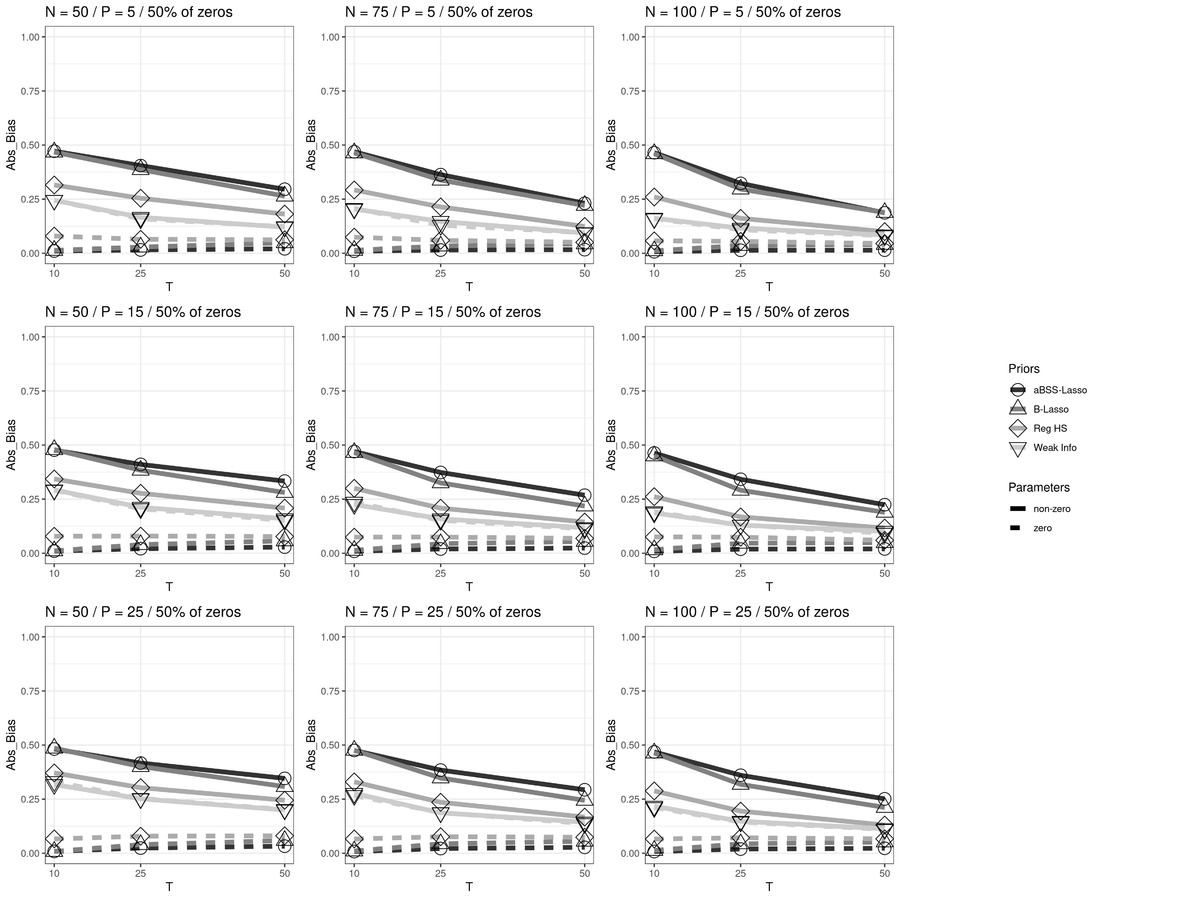
\includegraphics[width=18cm]{Abs_Bias_nz50_beta.jpg}
\caption{Absolute Bias across $N, T$ and $P$ slope when 50\% of $\beta$ components are zeros}
\end{figure}

\clearpage
\paragraph*{Relative Bias}
The relative bias of an estimator $\hat{\theta}_m$ of a parameter $\theta$ is computed by the following  quantity:
\[  RB = \frac{1}{M} \sum_{m=1}^{M} \dfrac{\hat{\theta}_m}{\theta} \]

\begin{figure}[h]\label{fig:RBias_nz25}
\centering 
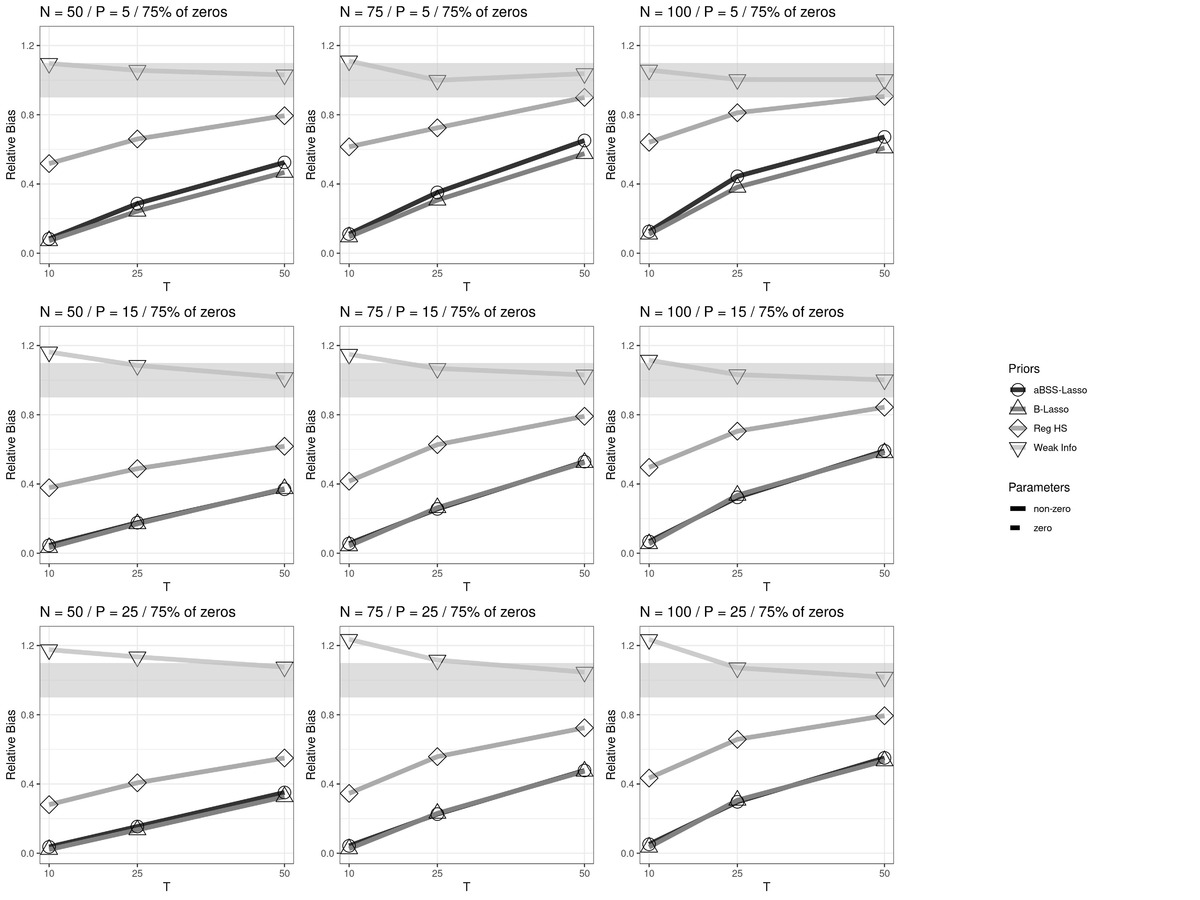
\includegraphics[width=18cm]{Rel_Bias_nz25_beta.jpg}
\caption{Absolute Bias across $N, T$ and $P$ slope when 75\% of $\beta$ components are zeros}
\end{figure}

\begin{figure}[]\label{fig:RBias_nz50}
\centering 
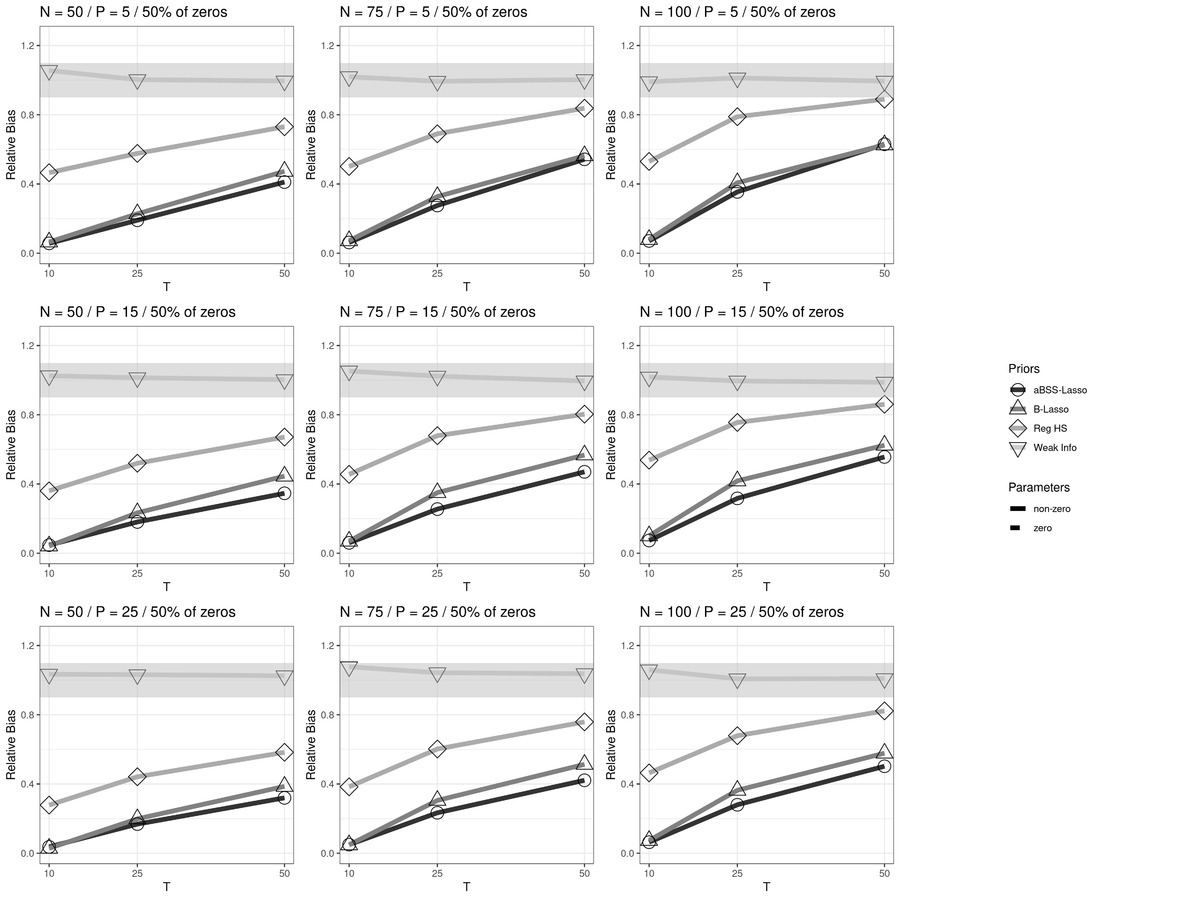
\includegraphics[width=18cm]{Rel_Bias_nz50_beta.jpg}
\caption{Absolute Bias across $N, T$ and $P$ slope when 50\% of $\beta$ components are zeros}
\end{figure}

\clearpage
\paragraph{RMSE}
The RMSE of an estimator $\hat{\theta}_m$ of a parameter $\theta$ is computed by the following  quantity:
\[  RMSE = \sqrt{\frac{1}{M}\sum_{m=1}^{M}(\theta-\hat{\theta}_m)^2} \]

\begin{figure}[h]\label{fig:MSE_nz25}
\centering 
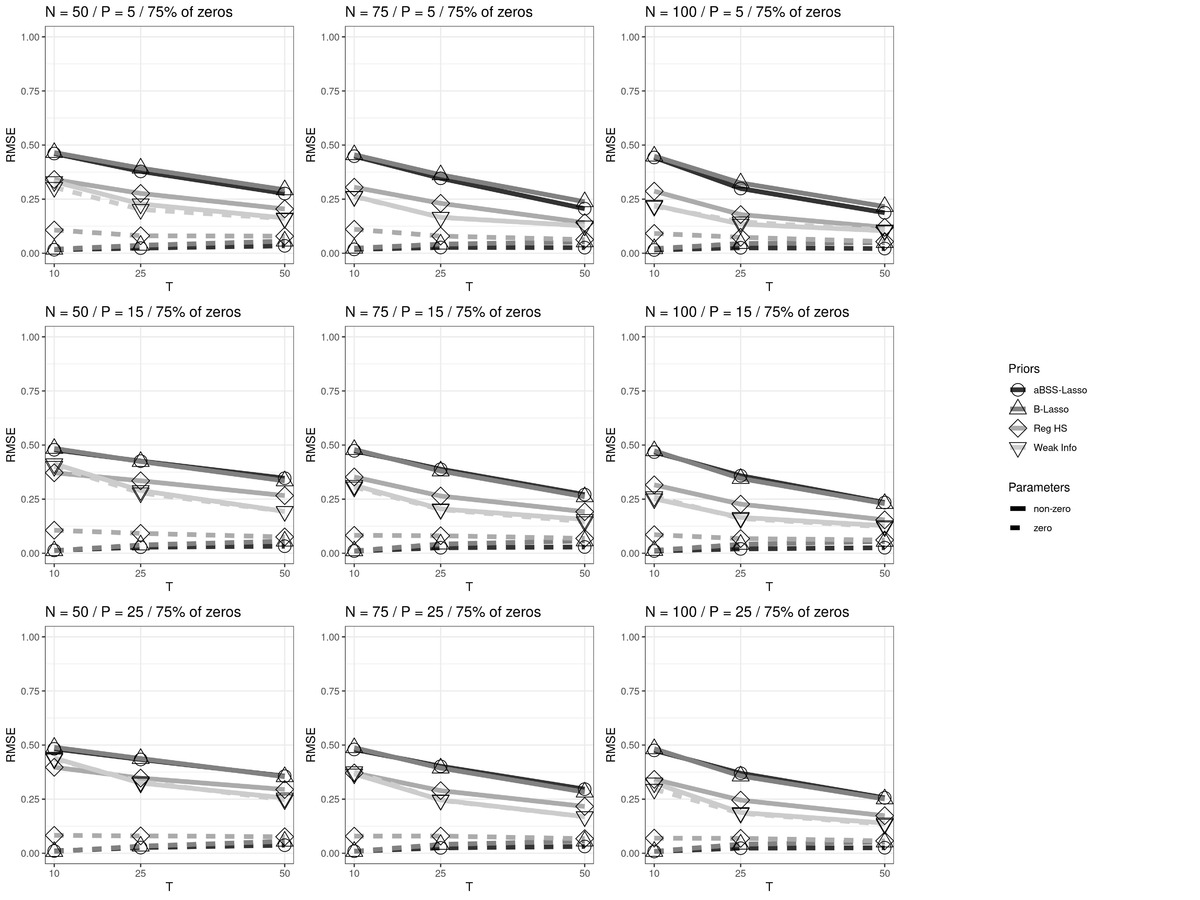
\includegraphics[width=18cm]{MSE_nz25_beta.jpg}
\caption{RMSE across $N, T$ and $P$ slope when 75\% of $\beta$ components are zeros}
\end{figure}

\begin{figure}[]\label{fig:MSE_nz50}
\centering 
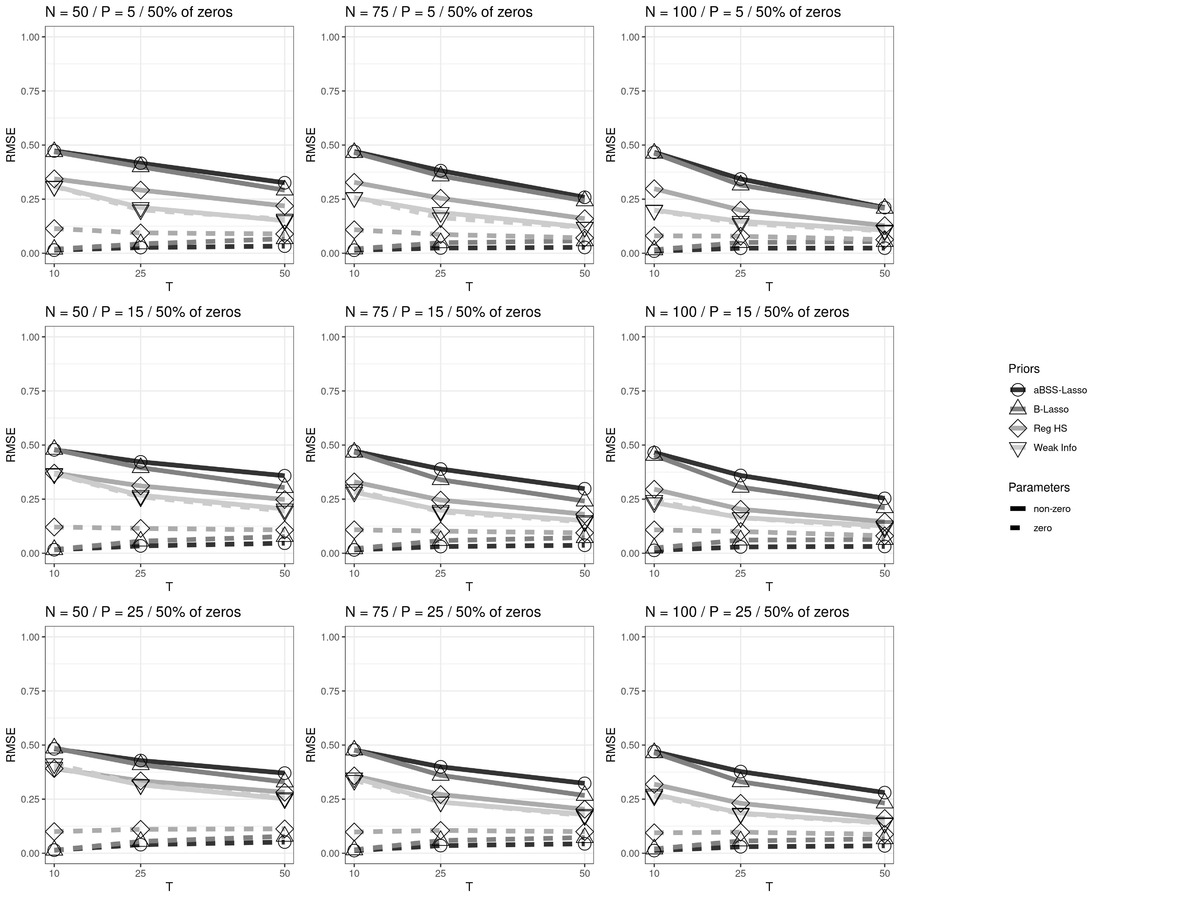
\includegraphics[width=18cm]{MSE_nz50_beta.jpg}
\caption{RMSE across $N, T$ and $P$ slope when 50\% of $\beta$ components are zeros}
\end{figure}

\clearpage
\paragraph{Coverage rates and Type-I-error rates}
The following figures show the Coverage rates and Type-I-error rates when 75\% of the $\beta$ components are zeros. 

\begin{figure}[h]\label{fig:CIR_nz25}
\centering 
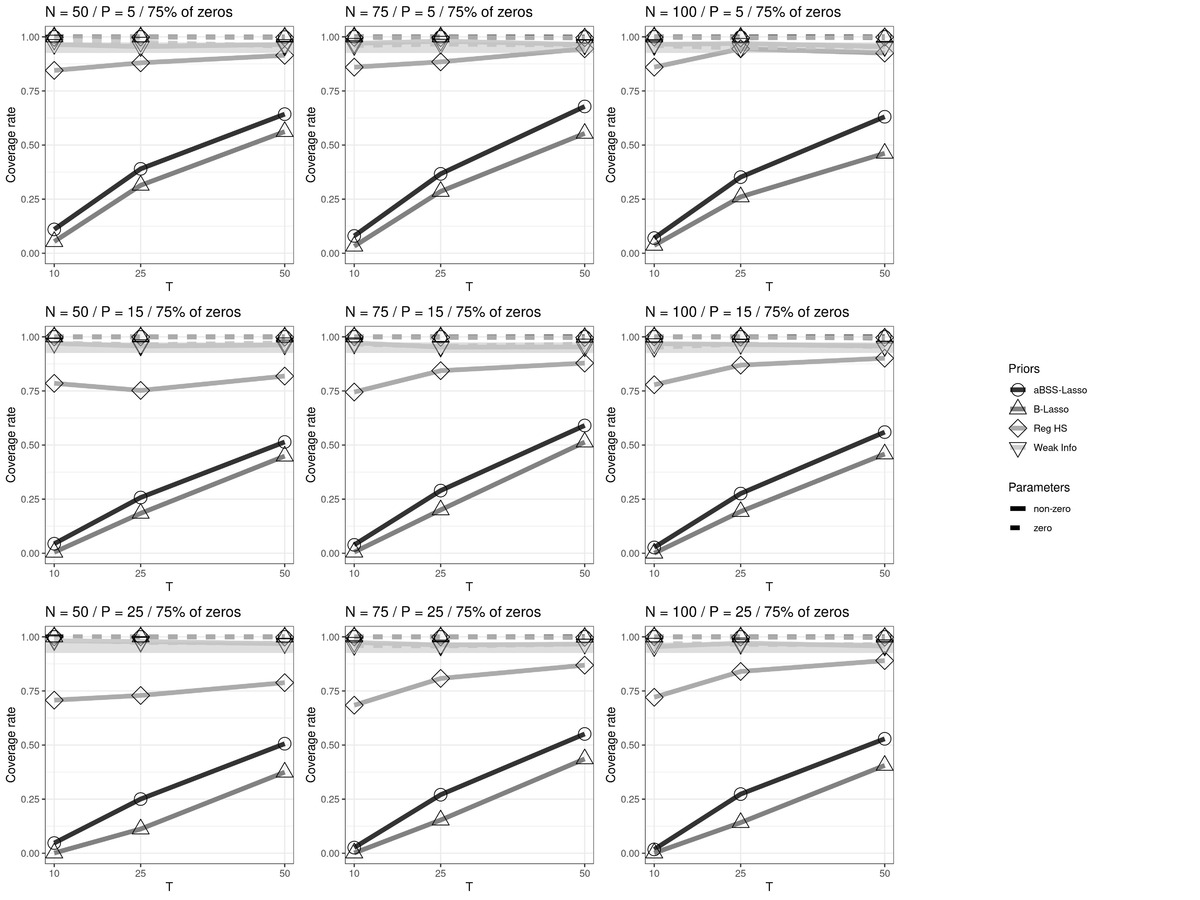
\includegraphics[width=18cm]{CIR_nz25_beta.jpg}
\caption{Coverage rates across $N, T$ and $P$ slope when 75\% of $\beta$ components are zeros}
\end{figure}

\begin{figure}[]\label{fig:NDR_nz25}
\centering 
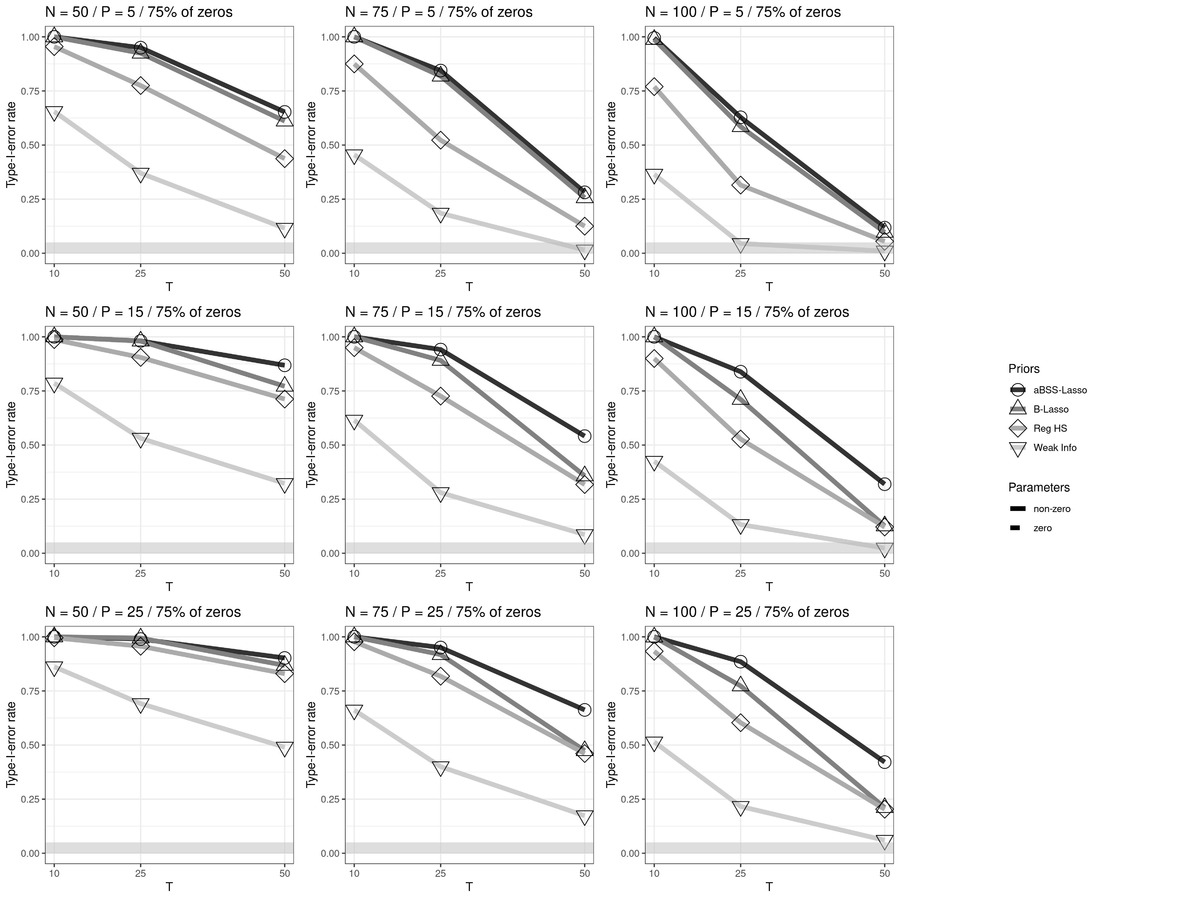
\includegraphics[width=18cm]{NDR_nz25_beta.jpg}
\caption{Type-I-error rates across $N, T$ and $P$ slope when 75\% of $\beta$ components are zeros}
\end{figure}

\clearpage
\section{Simulation study 2}

In this section, we present the sampling precision over the data conditions of Simulation Study 2. To compute this quantity we applied the same thresholds to ESS as in simulation study 1, i.e. $x=100,400,1000$. Figure \ref{fig:prec2} shows the corresponding results. 

When the threshold was $x=100$, the results showed that the weakly informative prior reached  precision rate of 100\%. In other words, all parameters produced 100 ESS across all replications and all data conditions. For the other priors, the lowest sampling precision rates were respectively: 98.5\% for the B-Lasso, 94\% for the Reg. HS and 81\% for the aBSS-Lasso. When the threshold was $x=400$, the weakly informative prior still provided a sampling precision rate of 100\%. For the the B-lasso, the lowest rate was 96.5\% and the highest was 100\%. For the Reg. HS, the lowest rate was 86\% and the highest was 92\%. For the aBSS-Lasso, the lowest rate was 68\% and the highest was 79\%. When the threshold was $x=1000$, the sampling rates for all priors decreased further. The B-Lasso prior had the best sampling rates with an average rate of 87.4\%. This is followed by the weakly informative prior with a sampling rate of 57.9\%. For the aBSS-Lasso and the Reg. HS priors, the average sampling rates were 51.8\% and 44.3\% respectively.   \\

\begin{figure}[h]
\centering 
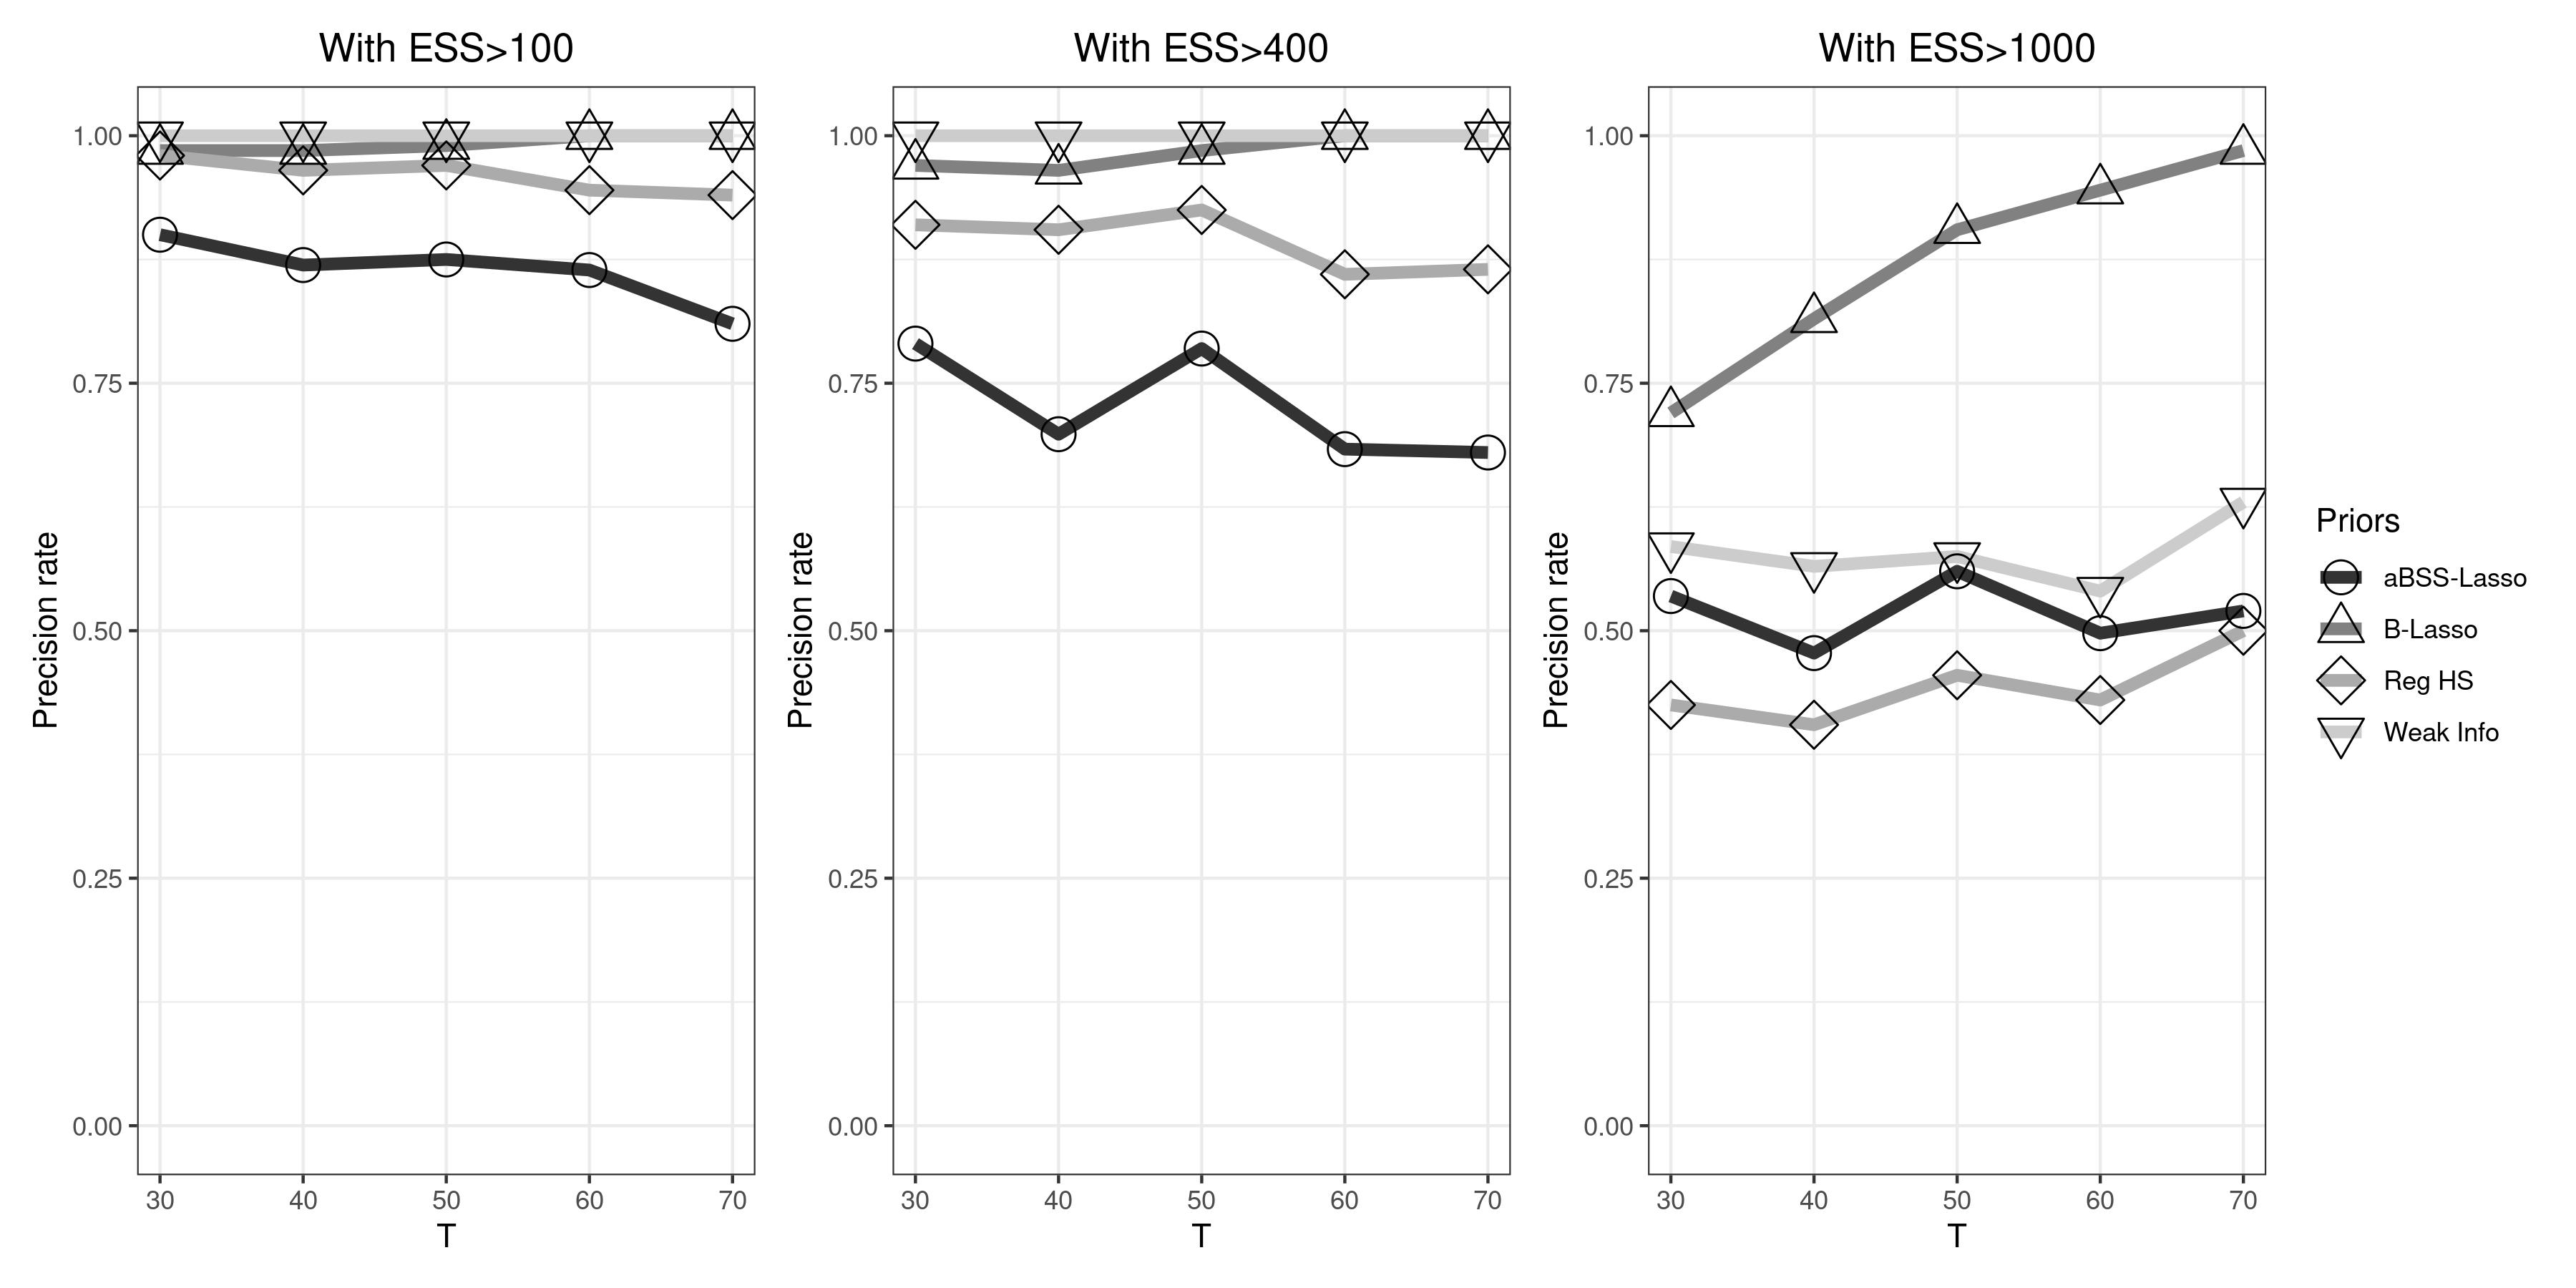
\includegraphics[width=15cm]{prec1004001000.jpg}
\caption{Comparison of the sampling precision rates for each prior distribution across different numbers of time points $T$. }
\label{fig:prec2}
\end{figure}


\end{document}




